\section{Distributed Bayesian Filter via FIFO Protocol}\label{sec:\proto-dbf}
	We first introduce the generic distributed Bayesian filter (DBF).
	%, which is also stated in \cite{bandyopadhyay2014distributed} and \cite{julian2012distributed}. 
	%Each UGV has its individual estimation of the probability density function (PDF) of target position, called \textit{individual PDF}. 
	Let $\X_k\in S$ be the random variable representing the position of the target at time $k$.
	Define $\Z^i_k$ as the set of measurements of time $k$ that are in the $i\thi$ UGV's CB, i.e., \small$\Z^i_k=\lb z^j_k| \left[x^j_k,z^j_k\right]\in \B^i_k,\; \forall j\in V\rb$\normalsize and let $\Z^i_{1:k} = \bigcup\limits_{t=1}^k \Z^i_t$. 
	We also define $z^i_{1:k}=\left[z^i_1,\dots,z^i_k\right]$ as the set of the $i\thi$ UGV's measurements of times $1$ through $k$.
%	\todohere{probably use $z^V_{1:k}$ here? And then use $z^i_{1:k}$ as the set for only UGV $i$.}
	The probability density function (PDF) of $\X_k$, called \textit{individual PDF}, of the $i\thi$ UGV is represented by
	%=\left\lbrace z^i_1,\dots,z^i_k\right\rbrace
	$P^i_{pdf}(\X_{k}|\Z^i_{1:k})$.
	It is the estimation of the target position given all the measurements that the $i\thi$ UGV has received.	
%	where $\mathbf{z}^i_{1:k}$ denotes the set of measurements by $i\thi$ UGV and by UGVs in $\mathcal{Q}_i$, that have been received by $i\thi$ UGV until time $k$.
	%by UGVs in $\mathcal{Q}_i$ that have been transmitted to $i\thi$ UGV by time $k$.
	%from time $1$ through $k$ and $z^{\mathcal{Q}_i}_{1:k}$ means the set of measurements by UGVs in $\mathcal{Q}_i$ that are transmitted to $i\thi$ UGV.
	%Note that if the measurement by $j\thi(j\in \mathcal{Q}_i)$ UGV at time $k'(k'\leq k)$ is not received by $i\thi$ UGV, the corresponding element $z^j_{k'}$ in $z^{\mathcal{Q}_i}_{1:k}$ is empty and thus not utilized for computing $i\thi$ individual PDF.
	The initial individual PDF, $P^i_{pdf}(\X_0)$, is constructed %=P(\X_0) $P^i_{pdf}(\X_0|\mathbf{z}^i_0)$
	%$P^i_{pdf}(x_0|z^i_0,z^{\mathcal{Q}_i}_0)=P(x_0)$, 
	given prior information including past experience and environment knowledge. 
	It is necessary to initialize $P^i_{pdf}(\X_0)$ such that the probability density of the true target position is nonzero, i.e., $P^i_{pdf}(\X_0=x^g_0)> 0$.
	
	Under the framework of DBF, the individual PDF is recursively estimated by two steps: the prediction step and the updating step. 
	%, based on measurements of $i\thi$ UGV and UGVs in $\mathcal{Q}_i$.
	
%	\subsubsection{Prediction}
	%The $i\thi$ individual PDF at time $k-1$ is known, denoted as $P^i_{pdf}(x_{k-1}|z^i_{1:k-1},z^{\mathcal{Q}_i}_{1:k-1})$. 
	%At time $k$, the prior individual PDF $P^i_{pdf}(x_{k-1}|z^i_{1:k-1},z^{\mathcal{Q}_i}_{1:k-1})$ is first predicted forward by using the Chapman-Kolmogorov equation:
	\textbf{Prediction.}
	At time $k$, the prior individual PDF $P^i_{pdf}(\X_{k-1}|\Z^i_{1:k-1})$ is first predicted forward by using the Chapman-Kolmogorov equation:
	%\small\begin{align}\label{eqn:bayes_pred}
	%&P^i_{pdf}(x_k|z^i_{1:k-1},z^{\mathcal{Q}_i}_{1:k-1})\notag\\
	%&=\int P(x_k|x_{k-1})P^i_{pdf}(x_{k-1}|z^i_{1:k-1},z^{\mathcal{Q}_i}_{1:k-1})dx_{k-1}
	%\end{align}\normalsize
	\small
	\begin{equation}\label{eqn:bayes_pred}
	P^i_{pdf}(\X_k|\Z^i_{1:k-1})
	=\int\limits_{\X_{k-1}\in S} P(\X_k|\X_{k-1})P^i_{pdf}(\X_{k-1}|\Z^i_{1:k-1})d\X_{k-1},
	\end{equation}\normalsize
	where $P(\X_k|\X_{k-1})$ represents the state transition probability of the target, based on the Markovian motion model (\Cref{eqn:tar_motion_model}). % from the prior position $\X_{k-1}$ to the posterior position $\X_k$, 
	% independent of UGV states. 
	%This model describes 
	%Note that the target is static in many search applications, such as the indoor search for stationary objects \cite{kulich2014single}. 
	%, as defined in \Cref{eqn:tar_motion_model},
%	For the deterministic motion model, the state transition probability is simplified to be
%	\small\begin{equation}\label{eqn:markov_model}
%	P(\X_k=c_k|\X_{k-1}=c_{k-1})=\begin{cases}
%	1 & \text{if}\quad c_k=f(c_{k-1})\\ %
%	0 & \text{otherwise}
%	\end{cases}.
%	\end{equation}\normalsize
	
%	\subsubsection{Updating}
	\textbf{Updating.}
	The $i\thi$ individual PDF is then updated by the Bayes' rule using the set of newly received measurements at time $k$, i.e., $\Z^i_k$:
%	\small \begin{equation}
%	P^i_{pdf}(\X_k|\Z^i_{1:k})= K_iP^i_{pdf}(\X_k|\Z^i_{1:k-1})P(\Z^i_k|\X_k)
%	\end{equation}\normalsize
	\begin{subequations}\label{eqn:bayes_upd}
		\small\begin{align}
%			\begin{split}
				P^i_{pdf}(\X_k|\Z^i_{1:k})
				&= K_iP^i_{pdf}(\X_k|\Z^i_{1:k-1})P(\Z^i_k|\X_k)\label{subeqn:bayes_upd_general}\\
				&=K_iP^i_{pdf}(\X_k|\Z^i_{1:k-1})\prod\limits_{z^j_k\in\Z^i_k}P(z^j_k|\X_{k})\label{subeqn:bayes_upd_factor},
%			\end{split}
		\end{align}\normalsize
	\end{subequations}
	where $P(z^j_k|\X_k)$ is the sensor model and $K_i$ is a normalization factor, given by:
	\small\begin{align*}
	K_i=\left[\int\limits_{\X_k\in S} P^i_{pdf}(\X_k|\Z^i_{1:k-1})P(\Z^i_k|\X_k)d\X_k\right]^{-1}.
	\end{align*}\normalsize
	\textcolor{orange}{Here we have utilized the commonly adopted assumption \cite{furukawa2006recursive,gu2007distributed,sheng2005distributed} in the distributed filtering literature that the measurements of each UGV at current time are conditionally independent from its own previous measurements and the measurements of other UGVs given the target and the UGVs' current positions.
	This assumption allows us to simplify $P(\Z^i_k|\X_k,\Z^i_{1:k-1})$ as $P(\Z^i_k|\X_k)$ in \Cref{subeqn:bayes_upd_general} and factorize $P(\Z^i_k|\X_k)$ as $\prod\limits_{z^j_k\in\Z^i_k}P(z^j_k|\X_{k})$ in \Cref{subeqn:bayes_upd_factor}.}
%	The factorization of $P(\Z^i_k|\X_k)$ comes from the conditional independence of measurements from each UGV given the target position and the corresponding UGV's position.	
	
	\begin{algorithm}
		\caption{\proto-DBF Algorithm}\label{alg:lifo-dbf}
		\begin{algorithmic}
			\State For $i\thi$ UGV at $k\thi$ step ($\forall i\in V$):
			%				\State After the updating step in \cref{alg:lifo},
			\State\textbf{(1)} Initialize a \textit{temporary PDF} by assigning the stored individual PDF to it:
			\small\begin{equation*}
			P^i_{tmp}(\X_{t})= P^i_{sto}(\X_t),
			%			P^i_{pdf}(\X_{k-N}|z^1_{1:k-N},\dots,z^N_{1:k-N}).
			\end{equation*}\normalsize		
			where % the stored individual PDF is for time $t$:
			\small\begin{equation*}
			P^i_{sto}(\X_t) = P^i_{pdf}(\X_{t}|z^1_{1:t},\dots,z^N_{1:t}).
			\end{equation*}\normalsize	
			\State\textbf{(2)} For $\xi=t+1$ to $k$, iteratively repeat two steps of Bayesian filtering:
			
			\State(2.1) Prediction 
			\small\begin{equation*}
			P_{tmp}^{pre}(\X_{\xi})=\int_{S} P(\X_{\xi}|\X_{\xi-1})P^i_{tmp}(\X_{\xi-1})d\X_{\xi-1}.
			\end{equation*} \normalsize
			
			\State(2.2) Updating
			%				\small\begin{gather*}
			%				P^i_{tmp}(\X_{\xi})=K_{\xi} P_{tmp}^{pre}(\X_{\xi})\prod\limits_{j\in\Omega^i_{\xi}}P(z^j_{\xi}|\X_{\xi}),\\
			%				K_{\xi}=\left[\int_S P_{tmp}^{pre}(\X_{\xi})\prod\limits_{j\in\Omega^i_{\xi}}P(z^j_{\xi}|\X_{\xi})d\X_{\xi}\right]^{-1}.
			%				\end{gather*} \normalsize
			\small\begin{gather*}
			P^i_{tmp}(\X_{\xi})=K_{\xi} P_{tmp}^{pre}(\X_{\xi})P(\Z^i_{\xi}|\X_{\xi}),\\
			K_{\xi}=\left[\int_S P_{tmp}^{pre}(\X_{\xi})P(\Z^i_{\xi}|\X_{\xi})d\X_{\xi}\right]^{-1}.
			\end{gather*} \normalsize
			
			\State(2.3)
			If $z^j_{\xi}\neq\emptyset$ for $\forall j\in V$, update the stored PDF:
			%				When $\xi=t+1$, if $z^j_{t+1}\neq\emptyset$ for $\forall j\in V$, update the stored PDF:
			%				then the stored PDF will be updated to be the temporary PDF of time $t+1$:
			\small\begin{equation*}
			P^i_{sto}(\X_{\xi})=P^i_{tmp}(\X_{\xi}).
			%		P^i_{pdf}(\X_{k-N+1}|z^1_{1:k-N+1},\dots,z^N_{1:k-N+1})=P^i_{tmp}(\X_{k-N+1}).
			\end{equation*}\normalsize
			%				where 
			%				\small\begin{equation*}
			%				P^i_{tmp}(\X_{t+1})=P^i_{pdf}(\X_{t+1}|z^1_{1:t+1},\dots,z^N_{1:t+1}).
			%				\end{equation*}\normalsize
			
			\State\textbf{(3)} The individual PDF of $i\thi$ UGV at time $k$ is
			$P^i_{pdf}(\X_{k}|\Z^{i}_{1:k})=P^i_{tmp}(\X_k)$.		
		\end{algorithmic}
	\end{algorithm}
	
	\subsection{The FIFO-DBF Algorithm}
	The generic DBF is not directly applicable to time-varying interaction topologies. 
	This is because changing topologies can cause intermittent and out-of-sequence arrival of measurements from different UGVs, giving rise to the OOSM problem.
	One possible solution is to ignore all measurements that are out of the temporal order.
	This is undesirable since this will cause significant information loss.
	Another possible remedy is to fuse all measurements by running the filtering algorithm from the beginning at each time step.
	This solution naturally causes excessive computational burden.
	To avoid both OOSM problem and unnecessary computational complexity, we add a new PDF, namely the \textit{stored PDF}, $P^{i}_{sto}(\X_t)$, that is updated from the $i\thi$ UGV's initial PDF by fusing the state-measurement pairs of \textit{all} UGVs up to a certain time $t\le k$.
	The choice of $t$ is described in \Cref{subsec:tracklist}.
	%	 that are in the $i\thi$ UGV's CB.	
	%	Therefore, the choice of $t$ needs to ensure that the $i\thi$ UGV has received the state-measurement pairs of times no greater than $t$ from all UGVs, which is described in \Cref{sec:tracklist} by using the track lists.
	The individual PDF, $P^i_{pdf}(\X_k|\Z^i_{1:k})$, is then computed by fusing the measurements from time $t+1$ to $k$ in the CB into $P^i_{sto}(\X_t)$, running the Bayesian filter (\Cref{eqn:bayes_pred,eqn:bayes_upd}).
	Note that initially, $P^{i}_{sto}(\X_0)$ = $P^i_{pdf}(\X_0)$.
	
	The \textbf{\proto-DBF algorithm} is stated in \cref{alg:lifo-dbf}.
	Each UGV runs \proto-DBF after its CB is updated in the Updating Step in \Cref{alg:lifo}.
	At the beginning, we assign the stored PDF to a temporary PDF, which will then be updated by sequentially fusing measurements in the CB to obtain the individual PDF.
	%	We use $\Omega^i_{\xi}\,\left(\xi=t+1,\dots,k\right)$ to denote the index set of UGVs whose state-measurement pair of time $(\xi)$ is stored in $i\thi$ UGV's CB, i.e. $\Omega^i_{\xi}=\left\lbrace j\in \mathcal{Q}_i \bigcup \left\lbrace i \right\rbrace | \left[x^j_\xi,z^j_{\xi}\right]\in B^i_k\rb$.
	%	The measurements will be sequentially used to update the temporary PDF until the latest measurements are used.
%	The temporary PDF is then assigned as the individual PDF of time $k$.
	It should be noted that, when the UGV's CB contains all UGVs' state-measurement pairs from $t$ to $\xi$, the temporary PDF of $\xi$ is assigned as the stored PDF.
	\cref{fig:LIFO-DBF} illustrates the \proto-DBF procedure for the $1^\text{st}$ UGV as an example.
	It can be noticed that, the purpose of using the stored PDF is to avoid running the Bayesian filtering from the initial PDF at every time step. 
	Since the stored PDF has incorporated all UGVs' measurements up to some time step $t$, the information loss is prevented. % when computing the individual PDF.
	%	each UGV only needs to start from the stored PDF each time it computes the individual PDF.
	We point out that the time $t$ of each UGV's stored PDF can be different from others.
	The stored PDF is saved locally by each UGV and not transmitted to others.
%	\footnote{\todohere{change notations here} Due to the space limit, in this figure we use $P^i_{pdf}(k)$, $P^i_{pdf}(k-N)$ and $P^i_{pdf}(k-N+1)$ to represent $P^i_{pdf}(\X|\mathbf{z}^{i}_{1:k})$ $P^i_{pdf}(\X|\mathbf{z}^{i}_{1:k-N})$ and $P^i_{pdf}(\X|\mathbf{z}^{i}_{1:k-N+1})$, respectively.}.
	
	\begin{figure}%[thpb]
		\centering
		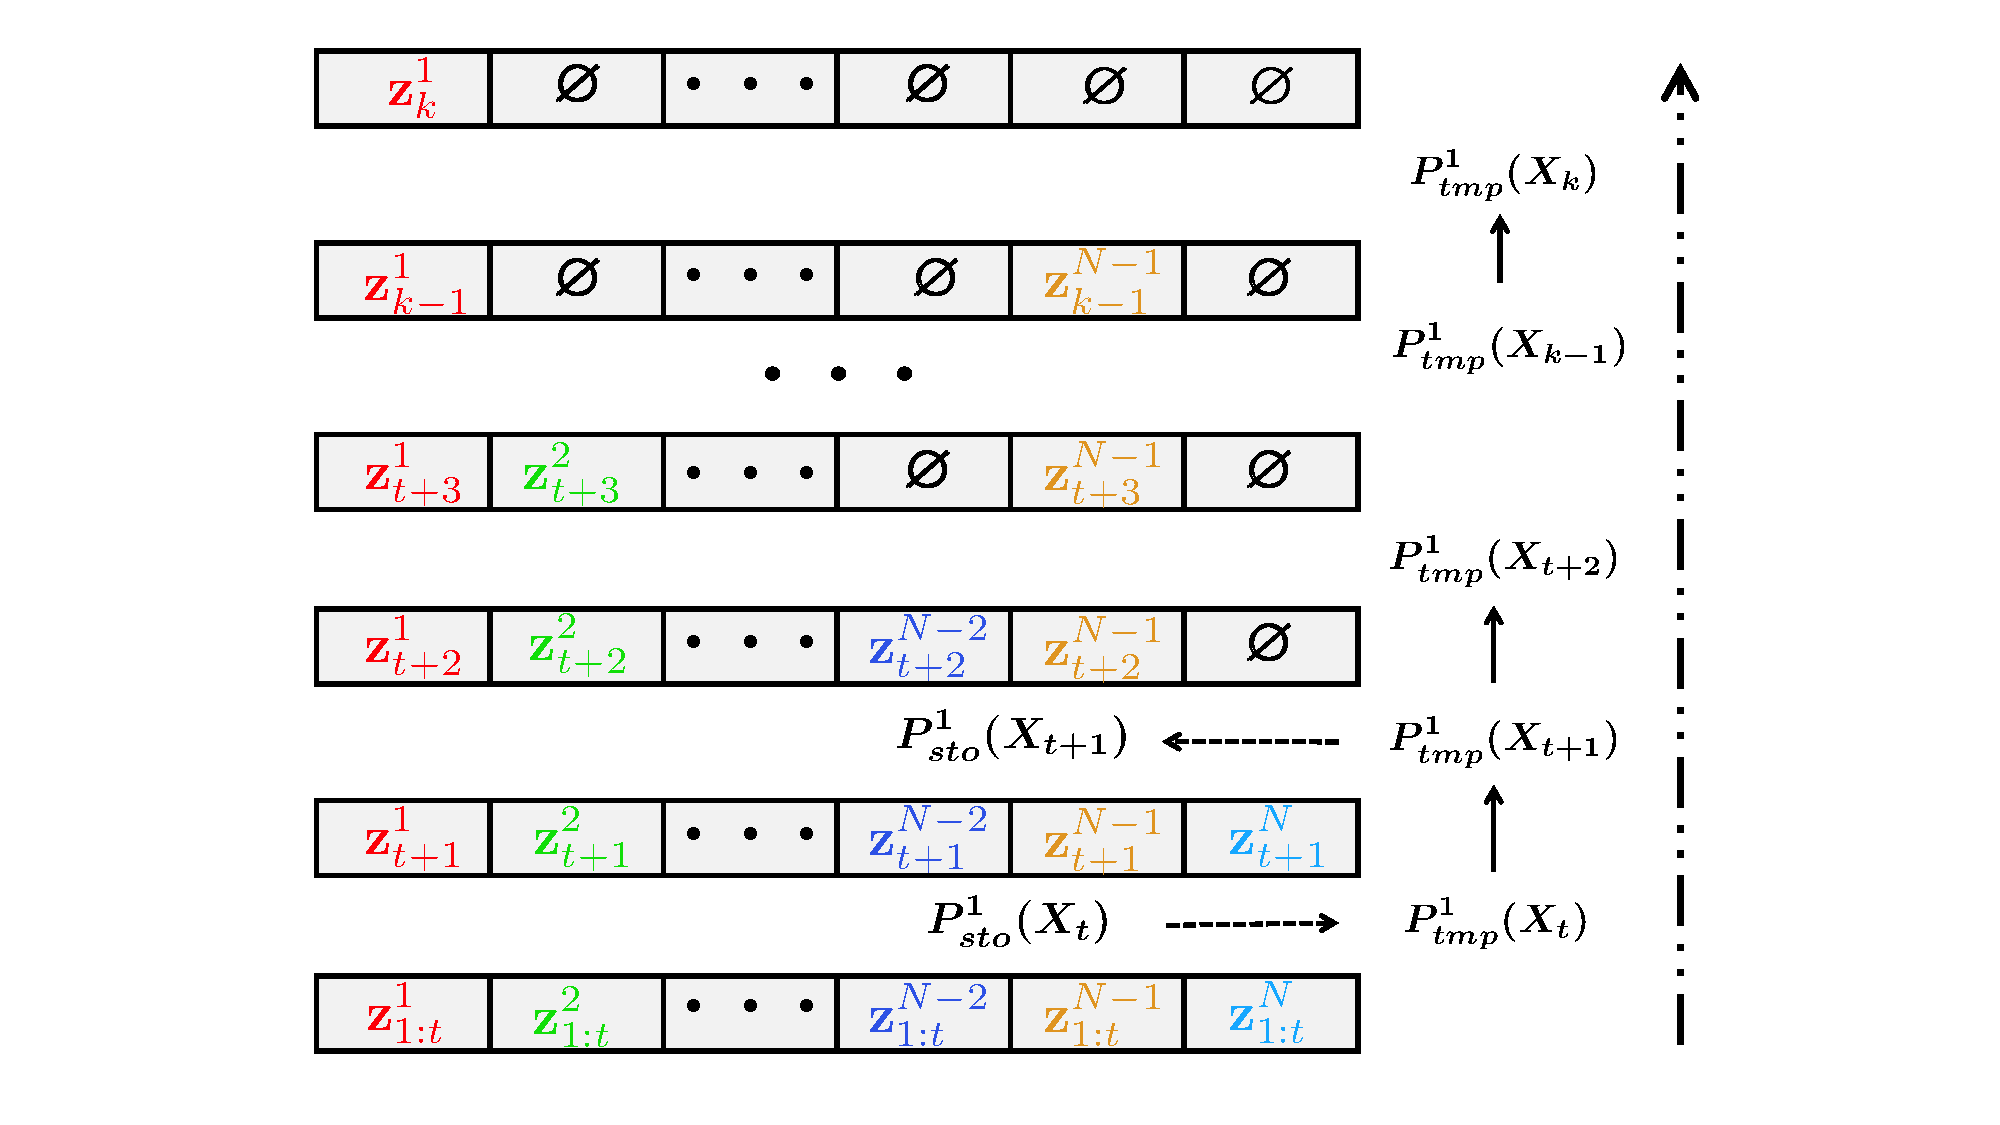
\includegraphics[width=0.50\textwidth]{figures/fifo-dbf}
		\caption{Example of \proto-DBF for the $1^\text{st}$ UGV at time $k$. 
			Only the measurement (not the state) is shown in the figure.
%			Networked UGVs take a line topology.
%			The stored individual PDF is represented by $ P^1_{pdf}(k-N)$.
			The UGV first calculates $ P^1_{tmp}(X_{t+1})$. 
			Since the UGV has received all UGVs' measurements of $t+1$, the $ P^1_{tmp}(X_{t+1})$ is assigned as the new stored PDF. 
			The dashed arrow on the right shows the order to fuse measurements in the CB.}
%			Repeating DBF until obtaining $ P^1_{pdf}(k)$.
			%		, which is the individual PDF at time $k$.
%			In this example, $\Omega^1_{\xi}=\left\lbrace 1,2,\dots,N+1-\xi\right\rbrace $, $\xi=1,\dots,N$.}
		\label{fig:LIFO-DBF}
%		\vspace{-1em}
	\end{figure}			
	
	\subsection{Track Lists for Trimming CBs}\label{subsec:tracklist}
	
	\begin{algorithm}
		\caption{Updating TLs}
		\label{alg:upd_tl}
		\begin{algorithmic}
			\State Consider updating the $i\thi$ UGV's TL, $\Q^i_k$, using the received $r\thi$ UGV's TL, $\Q^r_{k-1}(r\in \N^\text{in}_i(G_{k-1}))$.		
			\State \textbf{(1)} Update the $i\thi$ row of $\Q^i_k$, using $\B^i_k$:
			\begin{itemize}
				\item choose $k^{ii}$ as the minimum integer that satisfies the following conditions: (a) $\exists l\in V \text{ s.t. } \left[x^l_{k^{ii}},z^l_{k^{ii}}\right]\notin \B^i_k$ and (b) $k^{ii} \ge t_m-1$, where $t_m$ is the minimum time of state-measurement pairs in $\B^i_k$.
			\end{itemize}
			\State \textbf{(2)} Update other rows of $\Q^i_k$:
			$\forall j\in V\setminus\lb i\rb$
			\begin{itemize} 
				\item if $k^{ij}>k^{rj}$, keep current $\mathbf{q}^{ij}_{k^{ij}}$;
				\item if $k^{ij}=k^{rj}$, $\mathbf{q}^{ij}_{k^{ij}}=\mathbf{q}^{ij}_{k^{ij}} \lor\footnotemark\mathbf{q}^{rj}_{k^{rj}}$; 
				\item if $k^{ij}<k^{rj}$, $\mathbf{q}^{ij}_{k^{ij}}=\mathbf{q}^{rj}_{k^{rj}}$ and $k^{ij}=k^{rj}$.
			\end{itemize}
		\end{algorithmic}
	\end{algorithm}
	\footnotetext{`$\lor$' is the notation of the logical `OR' operator.}
	
	\begin{figure}%[thpb]
		\centering
		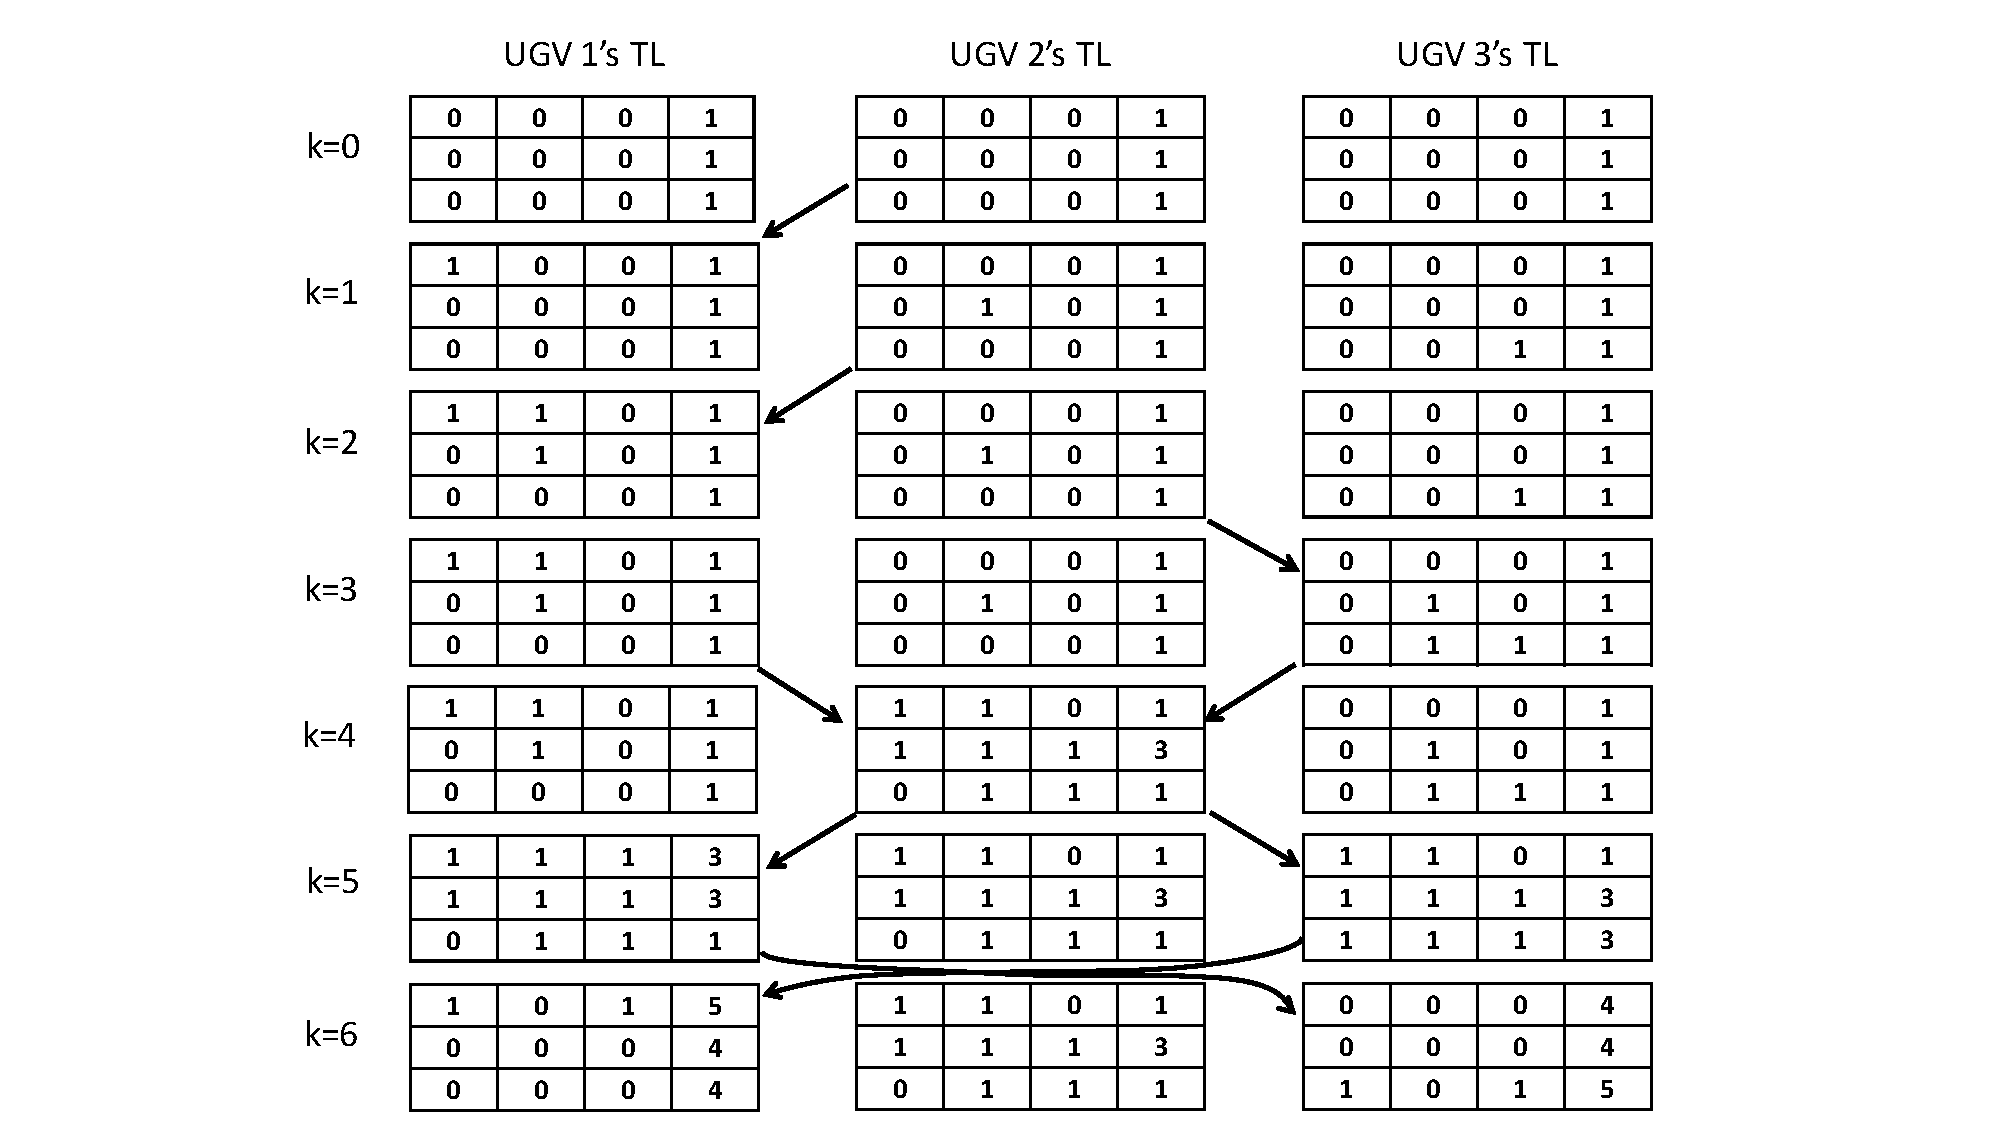
\includegraphics[width=0.50\textwidth]{figures/track_list}
		\caption{Example of updating TLs. For the $1^\text{st}$ UGV's TL, the $j\thi\,(j\in V)$ entry on the $i\thi\,(i\in V)$ row represents this UGV's knowledge about whether the $i\thi$ UGV has received the $j\thi$ UGV's state-measurement pair of time $k^{1i}$, where $k^{1i}$ is the last entry of the $i\thi$ row. TLs are updated using \cref{alg:upd_tl,alg:tracklist}.}
		\label{fig:upd_tl}
%		\vspace{-1em}
	\end{figure}
	
	The size of CBs can keep increasing as measurements cumulate over time. 
	The use of the stored PDF has made it feasible to trim excessive measurements from the CBs.
	%	while ensuring no information is lost in the sense that all UGVs' measurements have been used for update hte individual PDF.
	To avoid information loss, a state-measurement pair can only be trimmed from a UGV's CB when \textit{all} UGVs have received it.
	To keep track of each UGV's reception of other UGVs' measurements, every UGV maintains a \textit{track list} (TL), $\Q^i_k=\left[\mathbf{q}^{i1}_{k^{i1}},\dots, \mathbf{q}^{iN}_{k^{iN}}\right]^T \,(\forall i\in V)$, where $\mathbf{q}^{ij}_{k^{ij}}=\left[q^{j1}_{k^{ij}},\dots,q^{jN}_{k^{ij}},k^{ij}\right]^T$ ($j\in V$) is a $(N+1)\times 1$ binary vector.
	Therefore, a TL can be represented by a binary matrix of size $N\times (N+1)$, with the last column corresponding to the measurement time.
	$\Q^i_k$ represents the $i\thi$ UGV's knowledge of its own and other UGVs' measurements of the times specified by $k^{ij}\,(j\in V)$: %, in terms of the measurement time,
	the entry $q^{jl}_{k^{ij}}$ equals $1$ if the $i\thi$ robot knows that the $j\thi$ UGV has received the state-measurement pair of the $l\thi$ UGV of time $k^{ij}$, $\left[x^l_{k^{ij}},z^l_{k^{ij}}\right]$, and equals $0$ if the $i\thi$ robot cannot determine whether $\left[x^l_{k^{ij}},z^l_{k^{ij}}\right]$ has been received by the $j\thi$ robot, i.e.,
	%	\begin{equation*}
	%	q^{j,l}_{k^{j}}=
	%	\begin{cases}
	%	1 & \text{if}\quad \exists t\in\mathbb{N}, \text{ s.t. }k^{i,j}\le t\le k \text{ and } \left[x^l_{k^{i,j}},z^l_{k^{i,j}}\right]\in B^j_t,\\
	%	0 & \text{if}\quad \nexists t\in\mathbb{N}, \text{ s.t. }k^{i,j}\le t\le k \text{ and } \left[x^l_{k^{i,j}},z^l_{k^{i,j}}\right]\in B^j_t.
	%	\end{cases}
	%	\end{equation*}
	\small\begin{equation}\label{eqn:tl_entry}
	q^{jl}_{k^{ij}}=
	\begin{cases}
	1 & \text{if}\quad \exists t\in\left[k^{ij}, k\right] \text{ s.t. } \left[x^l_{k^{ij}},z^l_{k^{ij}}\right]\in \B^j_t,\\
	0 & \text{if}\quad \nexists t\in\left[k^{ij}, k\right] \text{ s.t. } \left[x^l_{k^{ij}},z^l_{k^{ij}}\right]\in \B^j_t.
	\end{cases}
	\end{equation}\normalsize
	Therefore it can happen that $\left[x^l_{k^{ij}},z^l_{k^{ij}}\right]$ has been received by the $j\thi$ UGV but the $i\thi$ UGV does not know this and thus $q^{jl}_{k^{ij}}=0$.
	
%	When all elements of $\Q^i_k$ are $1$'s, the $i\thi$ UGV can be sure that the $j\thi$ UGV ($\forall j\in V$) has received the state-measurement pairs of time $k^{i,j}$ from all UGVs.
	%	Choose the minimum time $k^i_m=\min\limits_j k^{i,j}$.
	%	Then the $i\thi$ robot fuse all the measurements of time no greater than $k^i_m$ in its own CB to update the stored PDF.
	%	TLs are exchanged when UGVs communicate and are used to trim the CBs. 
%	\todohere{rethink about how many steps a TL can be trimmed.}
	
	The exchange and updating of TLs are described in \Cref{alg:lifo}, with the updating details presented in \cref{alg:upd_tl}.
	For the $i\thi$ UGV, it updates the $i\thi$ row of its TL matrix using the entries of its CB, and updates other rows of the TL using the received TLs from {\inbhd}.
	The updating rule guarantees that, if the last term of the $j\thi$ row is $k^{ij}$, the $i\thi$ UGV is ensured that every UGV has received state-measurement pairs of times earlier than $k^{ij}$ from all UGVs.
	The \Cref{alg:tracklist} describes the approach to trim CBs using TLs.
%	Note that, due to the trimming of CBs, (2.3) in \Cref{alg:lifo-dbf} needs to be revised as follows:
%	
%	If $\xi<k^i_m$, then update the stored PDF:
%	\small\begin{equation*}
%	P^i_{sto}(\X_{\xi})=P^i_{tmp}(\X_{\xi}).
%	%		P^i_{pdf}(\X_{k-N+1}|z^1_{1:k-N+1},\dots,z^N_{1:k-N+1})=P^i_{tmp}(\X_{k-N+1}).
%	\end{equation*}\normalsize	
%	Since a TL only keeps track of the earliest measurements in CBs, the CBs are only trimmed by one time step each time the trim happens.
	\cref{fig:upd_tl} shows the updating of each UGV's TLs using the \cref{alg:upd_tl}.
	In the example, the $1^\text{st}$ and $3^\text{rd}$ UGV's CB will be trimmed at $k=6$ and the trimmed state-measurement pairs corresponds to times $1,2,$ and $3$.
	
	The use of TLs can avoid the excessive size of CBs and guarantee that trimming the CBs will not lose any information; the trimmed measurements have been encoded into the stored PDF.
	The following theorem formalizes this property.
	
	\begin{thm}\label{thm:trim_no_loss}
%		For a {\fc} network using FIFO-DBF, 
%		each UGV's individual PDF is updated with measurements from all UGVs. 
		Each UGV's estimation result using the trimmed CB is the same as that using the non-trimmed CB.
	\end{thm}
	
	\begin{proof}
%		According to \Cref{cor1}, each UGV receives the state-measurement pairs from all other UGVs within finite time steps that are used for updating the individual PDF.
		
		Consider the $i\thi$ UGV. Let $k^i_m=\min\limits_j k^{ij}$. 
		Trimming $\B^i_k$ happens when all entries in $\Q^i_k$ corresponding to time $k^i_m$ equal $1$. 
		This indicates that each UGV has received the state-measurement pairs of time $k^i_m$ from all UGVs.
%		, i.e., $\left[x^l_{k_m},z^l_{k_m}\right],\,l\in V$. 
		A UGV has either stored the pairs in its CB or already fused them to obtain the stored PDF.
		In both cases, such pairs are no longer needed to be transmitted. %since it will not add any unused information to the multi-agent team. 
		Therefore, it causes no loss to trim theses measurements.		
%		\hfill\qedsymbol
	\end{proof}
	
	%	Since TLs are used to reduce the size of CBs, it is necessary to understand how often the CBs will be trimmed.
%	The following theorem describes when CBs get trimmed.
	\textcolor{orange}{The following theorem describes when CBs get trimmed, and it provides an upper bound of the communication burden that FIFO will incur.
	A detailed complexity analysis of FIFO-DBF is presented in \Cref{subsec:complexity}.}
	Consider trimming all the state-measurement pairs of time $t$ in the $i\thi$ UGV's CB.
	Let $k^{lj}_t (>t)$ be the first time that the $l\thi$ UGV communicates to the $j\thi$ UGV in the time interval $(t,\infty)$.
	Define $\tilde{k}^j_t=\max\limits_l k^{lj}_t$, which is the time that the $j\thi$ UGV receives all other UGVs' measurements of $t$.
	Similarly, let $k^{ji}_t (> \tilde{k}^j_t)$ be the first time that the $j\thi$ UGV communicates to the $i\thi$ UGV in the time interval $(\tilde{k}^j_t,\infty)$ and define $\tilde{k}^i_t=\max\limits_j k^{ji}_t$.
	%	Let $d_{ji}$ is the shortest path distance from UGV $j$ to $i$ in the time interval $[t+d_{lj},t+d_{lj}+d_{ji}]$. 
	The following theorem gives the time when the $i\thi$ UGV ($\forall i\in V$) trims all state-measurement pairs of time $t$ in its own CB.
	\begin{thm}\label{thm:upd_tl_freq}		
		The $i\thi$ UGV trims $\lb\left[x^l_t,z^l_t\right] \,(\forall l\in V)\rb$ from its CB at the time $\tilde{k}^i_t$.
		%		interval $[\tilde{k}^i_t,t+2(N-1)T_u]$.
	\end{thm}
	
	\begin{proof}
%		We consider the case when the lower bound is achieved.
%		Assume that at time $t$ after the updating step, each UGV's CB only contains its own state-measurement pair of time $t$.
%		Then at $\tilde{k}_j$, the $j\thi$ UGV's CB has received all other UGVs' measurements at $t$.
		The $i\thi$ UGV can trim $\lb\left[x^l_t,z^l_t\right] \,(\forall l\in V)\rb$ only when it is sure that all other UGVs have also received these state-measurement pairs.
		This happens at $\tilde{k}^i_t$ and is thus the time when the trim occurs. 
		
%		\hfill\qedsymbol
		
		%		To compute the upper bound, we consider the time interval between the trims of time $t$ and $t+1$.\part{title}
		%		The largest interval is achieved when the CBs of all UGVs at $t$ are all empty
		
		%		The first time for the $j\thi$ UGV to receive $B^l_t$ from $l\thi$ UGV is time $t_{lj}$ and the $j\thi$ UGV's TL is updated so that $q^{j,l}_{t'}=1$ for some $t'\le t$.
		%		If $t'=t$, then all measurements before $t$ from the $l\thi$ UGV has already been fused to generate $P^j_{sto}(\X_{t-1})$. 
		%%		This is the case thus the shortest possible time to trim all the state-measurement pairs of $t$ in $i\thi$ UGV's CB.
		%		The first time the $i\thi$ UGV knows $g^{j,l}_{t'}=1$ is at time $k^{lji}_t$, when the $j\thi$ UGV's TL is transmitted to $i\thi$ UGV.
		%		Therefore, $\max\limits_{l,j\in V} k^{lji}_t$ is the earliest time when the $i\thi$ UGVs know about each UGV's reception of all measurements of time $t$.
		%				
		%		If $i\thi$ UGV's stored PDF corresponds to the time step $t-1$, then the trim happens at $k^i_t= \max\limits_{l,j\in V} k_t^{lji}$.
		%		If the stored PDF corresponds to a time step less than $t-1$, then the trim happens at $k^i_t> \max\limits_{l,j\in V} k_t^{lji}$.
		%		Therefore $k^i_t\ge \max\limits_{l,j\in V} k_t^{lji}$.
		%		The upper bound can be obtained using \Cref{prop1}.
	\end{proof}
	
	%	From \Cref{thm:upd_tl_freq}, we can get the following corollaries about how often the CB gets trimmed.
	
%	\begin{cor}
%		The first time to trim the $i\thi$ UGV's CB occurs at $\tilde{k}^i_1$.
%	\end{cor}
%	
%	\begin{proof}
%		%		The proof is straightforward by setting $t=1$ in the proof of \Cref{thm:upd_tl_freq} and 
%		Notice that the initial stored PDF of each UGV corresponds to the time $0$.
%		Therefore, the first time a TL is all $1$'s the trim occurs.
%	\end{proof}	
	
%	Under the \fc ness condition, the size of each UGV's CB is bounded.
%	\begin{thm}
%		The maximum interval between two consecutive trims is no greater than $T_M$.
%	\end{thm}
%	\begin{proof}
%		See the Appendix.
%	\end{proof}
	
	\begin{cor}\label{thm:max_CB_size}
		Under the \fc ness condition, the size of any UGV's CB is no greater than $2N(N-1)T_u$.
	\end{cor}
	
	\begin{proof}
		We consider an arbitrary $i\thi\,(i\in V)$ UGV.
		According to \Cref{prop1}, a UGV can communicate to any other UGV within $NT_u$ steps.
		Therefore, $\tilde{k}^i_t\le 2NT_u$, since it first requires each UGV communicate to all other UGVs and then each UGV communicate to the $i\thi$ UGV.
		This implies that, the state-measurement pairs of a certain time of all UGVs will be trimmed from each UGV's CB within $2NT_u$ steps.

		The maximum size the of CB occurs when the state-measurement pairs of a certain time from all but one UGV are saved in the $i\thi$ UGV's CB.
		Therefore, the size of any UGV's CB is no greater than $2N(N-1)T_u$.		
		
%		\hfill\qedsymbol
	\end{proof}
	
%	\begin{proof}
%		
%		Consider the time intervals $\left[k_m,k_{m+1} \right),\,m=1,2,\dots$ that are {\fc}, where $k_1=0$.
%		Define $\Delta_m = k_{m+1}-k_m,\,m=1,2,\dots$.
%		It is easy to know that $\Delta_i\le T_u$.
%		At $k_2$, the worst-case size of a UGV's CB is $(N-1)\Delta_1$.	
%		This can occur if UGVs do not communicate with each other until at $k_2$, when a UGV communicates with all others except one.
%		At $k_3$, according to the definition of a {\fc} network, every UGV has received measurements made at or before time $k_2$ from all UGVs.
%		The worst-case size of a UGV's CB is then $max \left[(N-1)(\Delta_2-\Delta_1),N(\Delta_1-\Delta_2)\right]$.  %$\Delta_2 = max(k_3-k_2-\Delta_1,0)$.
%		The first term is the worst-case size if $\Delta_2\ge\Delta_1$ and can be achieved similarly to the case of the time interval $\left[k_1,k_2\right)$. 
%		The second term corresponds to the worst-case size when $\Delta_1>\Delta_2$ and can be achieved if a UGV can receive measurements from all other UGVs in the whole time interval $\left[k_2,k_3\right)$. 
%		In general, at $k_{m+1}$, each UGV has already received all UGVs' measurements made at or before time $k_m$. 
%		The worst-case size of a UGV's CB within the time interval $\left[k_m,k_{m+1}\right)$ is $max\left[(N-1)(\Delta_m-\Delta_{m-1}),N(\Delta_{m-1}-\Delta_m)\right]$.
%		Since $\Delta_m\le T_u,\, m=1,2,\dots$, we know that the maximum CB size of each UGV is no greater than $NT_u$.
%	\end{proof}
	
	%	\begin{cor}
	%		The time between two consecutive trims of the $i\thi$ UGV's CB is 
	%		\begin{equation*}
	%			\Delta k_i=\begin{cases}
	%			1+n'_{i,t+1}-n_{i,t}& \text{if}\;n'_{i,t+1} \ge n_{i,t}\\
	%			1& \text{if}\;n'_{i,t+1} < n_{i,t}
	%			\end{cases},
	%		\end{equation*}
	%		where $n_{i,t}=\max\limits_{l,j}t_{ji}$ starting from $t$ and $n'_{i,t+1}=\max\limits_{l,j}t_{ji}$ starting from $t+1$.
	%	\end{cor}
	%	
	%	\begin{proof}
	%		Let $k_i = t+1+n_i$ and $k'_i = t+n'_i$ be the two consecutive trimming times.
	%		Since earlier measurements are always trimmed before the later measurements, this guarantees $\Delta k \ge 1$. 
	%		If $n'_i \ge n_i$, then it takes longer time for the later measurements to be trimmed and thus $\Delta k = 1+n_i'-n_i$.
	%	\end{proof}
	
	\begin{algorithm}
		\caption{Trimming CBs using TLs}
		\label{alg:tracklist}
		\begin{algorithmic}
			\State 
			For the $i\thi$ UGV:			
			find the smallest time in $\Q^i_k$: $k^i_m=\min\lb k^{i1},\dots,k^{iN} \rb$. 
			\begin{enumerate}
				\item Remove state-measurement pairs in $\B^i_k$ that corresponds to measurement times earlier than $k^i_m$, i.e., $\B^i_k=\B^i_k\setminus \lb\left[x^l_t,z^l_t\right] \rb,\,\forall t< k^i_m, \forall l\in V.$
				\item If entries associated with time $k^i_m$ in $\Q^i_k$ are $1$'s, then 
				\begin{enumerate}
					\item set these entries to be $0$.
					\item update the $i\thi$ row of $\Q^i_k$ using the current CB, i.e., $q^{il}_{k^{ij}}=1$ if $\left[x^l_{k^{ij}},z^l_{k^{ij}}\right]\in \B^i_k,\,\forall l\in V$.
					\item remove all corresponding state-measurement pairs in $\B^i_k$, i.e., $\B^i_k=\B^i_k\setminus \lb\left[x^l_{k^i_m},z^l_{k^i_m}\right] \rb,\, \forall l\in V.$
					\item $k^i_m \leftarrow k^i_m+1.$
				\end{enumerate}	
			\end{enumerate}				
		\end{algorithmic}
	\end{algorithm}
	
	\subsection{Complexity Analysis of FIFO-DBF}\label{subsec:complexity}
	Compared to statistics dissemination, {\proto} is usually more communication-efficient for distributed filtering. 
	To be specific, consider a grid representation of the environment with the size $D\times D$. %with a network of $N$ UGVs, 
	The transmitted data between each pair of UGVs are the CB and TL of each UGV.
	%	 and the corresponding UGV positions where observations were made, the length of which is $O(N)$. 
	The size of the CB is upper bounded by $O(N^2T_u)$, according to \Cref{thm:max_CB_size}.
%	$O(NT_M)$, according to \Cref{thm:max_CB_size}, and the size of the TL is $O(N^2)$.
%	Since $T_M\le (N-1)T_u)$, the overall communication complexity is upper bounded by $O(N^2T_u)$.	
	On the contrary, the communicated data of a statistics dissemination approach that transmits unparameterized posterior distributions or likelihood functions is $O(D^2)$.
	%	, which is in the order of environmental size. 
	In applications such as the target localization, $D$ is generally much larger than $N$ and the consensus filter usually requires multiple rounds to arrive at consensual results.
	Therefore, when $T_u$ is not comparable to $D^2$, the {\proto} protocol requires much less communication burden.
	
	%	It is worth noting that, for the static target, each UGV only needs current-step CB to update individual PDFs. 
	%	Therefore, besides storing its own individual PDF of size $O(M^2)$, only current-step CB of size $O(N)$ is stored in an UGV's memory and all previous CBs can be discarded, which means that the size of needed memory is $O(N+M^2)$. 
	%	On the contrary, for the moving target, 
	It is worth noting that each UGV needs to store an individual PDF and a sotred PDF, each of which has size $O(D^2)$. 
	In addition, each UGV needs to keep the CB and TL.
	%	Therefore the size of the needed memory for each UGV is $O(M^2+N^2)$.
	This is generally larger than that of statistics dissemination-based methods, which only stores the individual PDF.
	%	Besides, additional computation power is needed for LIFO-DBF compared to statistics dissemination-based methods.
	Therefore, the \proto-DBF sacrifices the local memory for reducing the communication burden. 
	This is actually desirable for real applications as local memory of vehicles is usually abundant compared to the limited bandwidth for communication.
	
	%	\begin{rem}
	%		We can change TLs to track measurements of multiple time steps so that CBs might be trimmed off multiple time steps at each trim.
	%		This, however, requires larger communication resource.
	%		The maximum size of CBs transmitted by UGVs is $O(NT_m)$, where $T_m=\max\limits_{l,j,i}\lb d_{lj}+d_{ji}\rb$ and $T_m\le NT_u$.
	%	\end{rem}	
	
	\begin{rem}
		Under certain interaction topologies, CBs can grow to undesirable sizes and causes excessive communication burden if the trim cannot happen frequently.
		In this case, we can use a time window to constrain the measurements that are saved in CBs.
		This will cause information loss to the measurements.
		However, with a decently long time window, FIFO-DBF can still effectively estimate the target position.
	\end{rem}